\section{Theoretical background and literature review}
\label{section:2}

\subsection{Rarefied flow}
The expression rarefied flow refers to a set of flow conditions where the gas is so rarefied that the continuum assumption of ordinary fluid mechanics ceases to be valid \cite{aerothermonotes}. Because of this, statistical mechanics has to be employed to describe it, rather than continuum mechanics.

It is possible to determine whether a flow is rarefied through the Knudsen number, a dimensionless number defined as in \autoref{eq:knudsen}, where $\lambda$ is the mean free path of the flow molecules and $l$ is a characteristic length of the flow.
\begin{equation}
    Kn=\frac{\lambda}{l}
    \label{eq:knudsen}
\end{equation}
As it is possible to see from \autoref{fig:regimes}, flows can be divided into three categories based on Knudsen number:
\begin{figure}[ht]
    \centering
    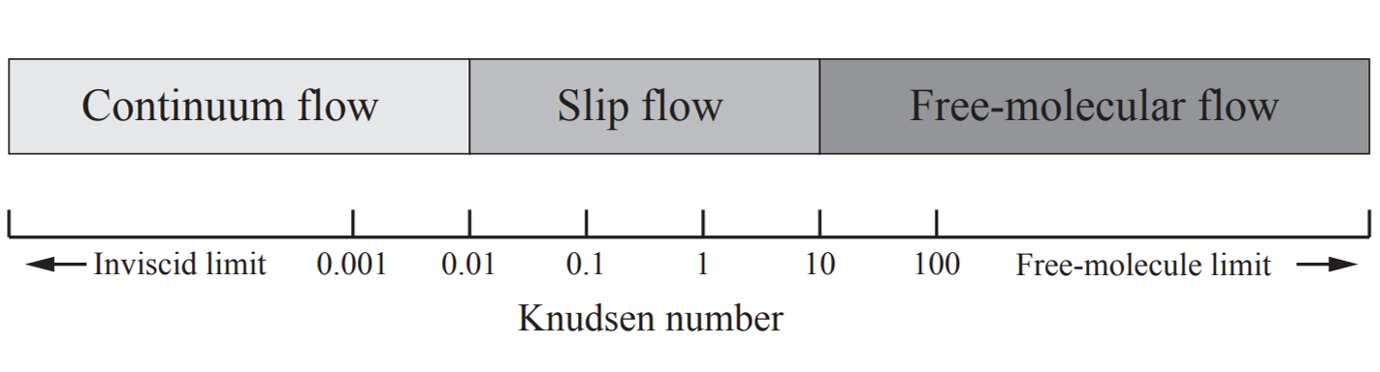
\includegraphics[width=0.7\textwidth]{../Images/2. Background/regimes.png}
    \caption{Flow regime with varying Knudsen number \cite{aerothermonotes}.}
    \label{fig:regimes}
\end{figure}
\begin{itemize}
    \item For Knudsen numbers below 10\textsuperscript{-2}, the flow can be classified as continuum. This kind of flow is characterised with a very significant number of intermolecular collision \cite{aerothermonotes, chambrerarefied}, and is commonly observed in everyday conditions, such as the flow around the wing of an aircraft or the flow of water in a pipe. It can be mathematically modelled through the Navier-Stokes equations.
    \item For Knudsen numbers between 10\textsuperscript{-2} and 10\textsuperscript{1}, flow can be classified as slip. In this condition the number of collisions between molecules is low, but not negligible \cite{chambrerarefied}. This leads to notable phenomena such as the boundary temperature jump, where the flow temperature at the wall differs from the surface wall temperature \cite{slipjump}. Moreover, a boundary slip velocity condition arises, which negates the the no-slip condition observed in ordinary flows \cite{slipjump}. These phenomena are schematically represented in \autoref{fig:slipjump}. The modelling of this regime depends on $Kn$. For conditions which approach the continuum flow, this regime can be modeled by incorporating correction factors into the Navier stokes equations \cite{slipjump} (in order to account for the aforementioned phenomena). Alternatively, it can be described through the Burnett and super Burnett equations \cite{burnett}.
    \item For Knudsen numbers above 10\textsuperscript{1}, the flow is classified as free molecular flow. In this regime, intermolecular collisions are so rare that the notion of an ordered flow of molecules ceases to exist \cite{aerothermonotes, chambrerarefied}, and is replaced by a statistical description, in the form of the Boltzmann equation.
\end{itemize}
\begin{figure}[ht]
    \centering
    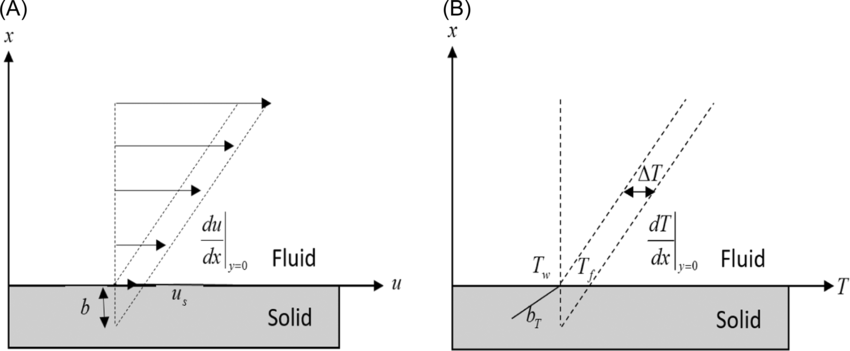
\includegraphics[width=0.7\textwidth]{../Images/2. Background/slipjump.png}
    \caption{Schematic diagram of velocity slip (A) and temperature jump (B)  \cite{slipjump}.}
    \label{fig:slipjump}
\end{figure}
It is important to note that while a flow may be globally continuous, certain local regions may exhibit signs of rarefied flow. An illustrative example of this phenomenon is the re-entry path of the space shuttle. While the global Knudsen number, calculated based on the length of the vehicle, may fall within the continuum regime, the Knudsen number associated with the flow around one of the rivets on its wing could differ significantly, potentially resulting in a different flow regime altogether.

ADD HATHORAERO2

\subsection{Rarefied flow mathematical modelling}
As mentioned previously, Navier-Stokes equations cease to be valid in the rarefied flow regime. Different methods thus need to be employed for its analytical description.

Free molecular flow is modelled through the Boltzmann equation, presented in \autoref{eq:boltzmann}. This equation, developed by Ludwig Boltzmann in 1872, describes the statistical behaviour of a thermodynamic system not in a state of equilibrium. The description that it gives is in terms of microscopic quantities, such as momentum $\mathbf{p}$ and mass $m$ of the particles, and is based on a particle distribution function $f (\mathbf{x}, \mathbf{c},t)$, which expresses the probability of finding a molecule in a volume $d\mathbf{x}$ with velocity between $\mathbf{c}$ and $\mathbf{c} + d \mathbf{c}$ \cite{burnett}.
\begin{equation}
    \frac{\partial f}{\partial t}+\frac{\mathbf{p}}{m} \cdot \nabla f+\mathbf{F} \cdot \frac{\partial f}{\partial \mathbf{p}}=\left(\frac{\partial f}{\partial t}\right)_{\text {coll }}
    \label{eq:boltzmann}
\end{equation}
While this description results provides an accurate representation of the system, it results to rather complex, because of its use of microscopic quantities. Therefore, a more convenient approach would be to employ a macroscopic description of the flow, in terms of common aerodynamic quantities, such as density and flow velocity.

To solve this problem, it is possible to assume small deviations from the equilibrium conditions, and apply an expansion to the Maxwell-Boltzmann particle distribution function. This expansion is denominated the Chapman-Enskog theory \cite{burnett}, and can be seen in \autoref{eq:chapman}.
\begin{equation}
    f=f^{(0)}+f^{(1)}+f^{(2)}+\cdots=\sum_{r=0}^{\infty} f^{(r)}
    \label{eq:chapman}
\end{equation}
It is thus possible to substitute this series expansion into the Boltzmann equation, obtaining:
\begin{itemize}
    \item For a zeroth order approximation, the Euler equations of motion (accurate to order 0 in Knudsen number)
    \item For a first order approximation, the Navier-Stokes equations (accurate to order 1 in Knudsen number)
    \item For a second order approximation, the Burnett equations (accurate to order 2 in Knudsen number and shown in \autoref{eq:burnett1} and \autoref{eq:burnett2})
    \item For a third order approximation, the Super Burnett equations (accurate to order 3 in Knudsen number)
\end{itemize}
\begin{equation}
    \begin{aligned}
        P_{i j}^{(2)}=\omega_1 \frac{\mu^2}{p} \frac{\partial u_k}{\partial x_k} S_{i j}+\omega_2 \frac{\mu^2}{p}\left\{\frac{\partial}{\partial x_{\langle i}}\left(F_{j\rangle}-\frac{1}{\rho} \frac{\partial p}{\partial x_{j\rangle}}\right)-\frac{\partial u_k}{\partial x_{\langle i}} \frac{\partial u_{j\rangle}}{\partial x_k}\right.  \left.-2 \frac{\partial u_k}{\partial x_{\langle i}} S_{j\rangle k}\right\} \\
        \quad + \omega_3 \frac{\mu^2}{\rho T} \frac{\partial^2 T}{\partial x_{\langle i} \partial x_{j\rangle}}+\omega_4 \frac{\mu^2}{p \rho T} \frac{\partial T}{\partial x_{\langle i}} \frac{\partial p}{\partial x_{j\rangle}}+\omega_5 \frac{\mu^2}{\rho T^2} \frac{\partial T}{\partial x_{\langle i}} \frac{\partial T}{\partial x_{j\rangle}} +\omega_6 \frac{\mu^2}{p} S_{k\langle i} S_{j\rangle k}
    \end{aligned}
    \label{eq:burnett1}
\end{equation}

\begin{equation}
    \begin{aligned}
        q_i^{(2)}  =\theta_1 \frac{\mu^2}{\rho T} \frac{\partial u_k}{\partial x_k} \frac{\partial T}{\partial x_i}+\theta_2 \frac{\mu^2}{\rho T}\left\{-\frac{2}{3} \frac{\partial}{\partial x_i}\left(T \frac{\partial u_k}{\partial x_k}\right)-2 \frac{\partial u_k}{\partial x_i} \frac{\partial T}{\partial x_k}\right\} \\
         +  \theta_3 \frac{\mu^2}{\rho p} S_{i k} \frac{\partial p}{\partial x_k}+\theta_4 \frac{\mu^2}{\rho} \frac{\partial S_{i k}}{\partial x_k}+3 \theta_5 \frac{\mu^2}{\rho T} S_{i k} \frac{\partial T}{\partial x_k}
    \end{aligned}
    \label{eq:burnett2}
\end{equation}

More details about the derivations can be seen in the flowchart in \autoref{fig:flowchart} and in \cite{burnett}.

\begin{figure}[ht]
    \centering
    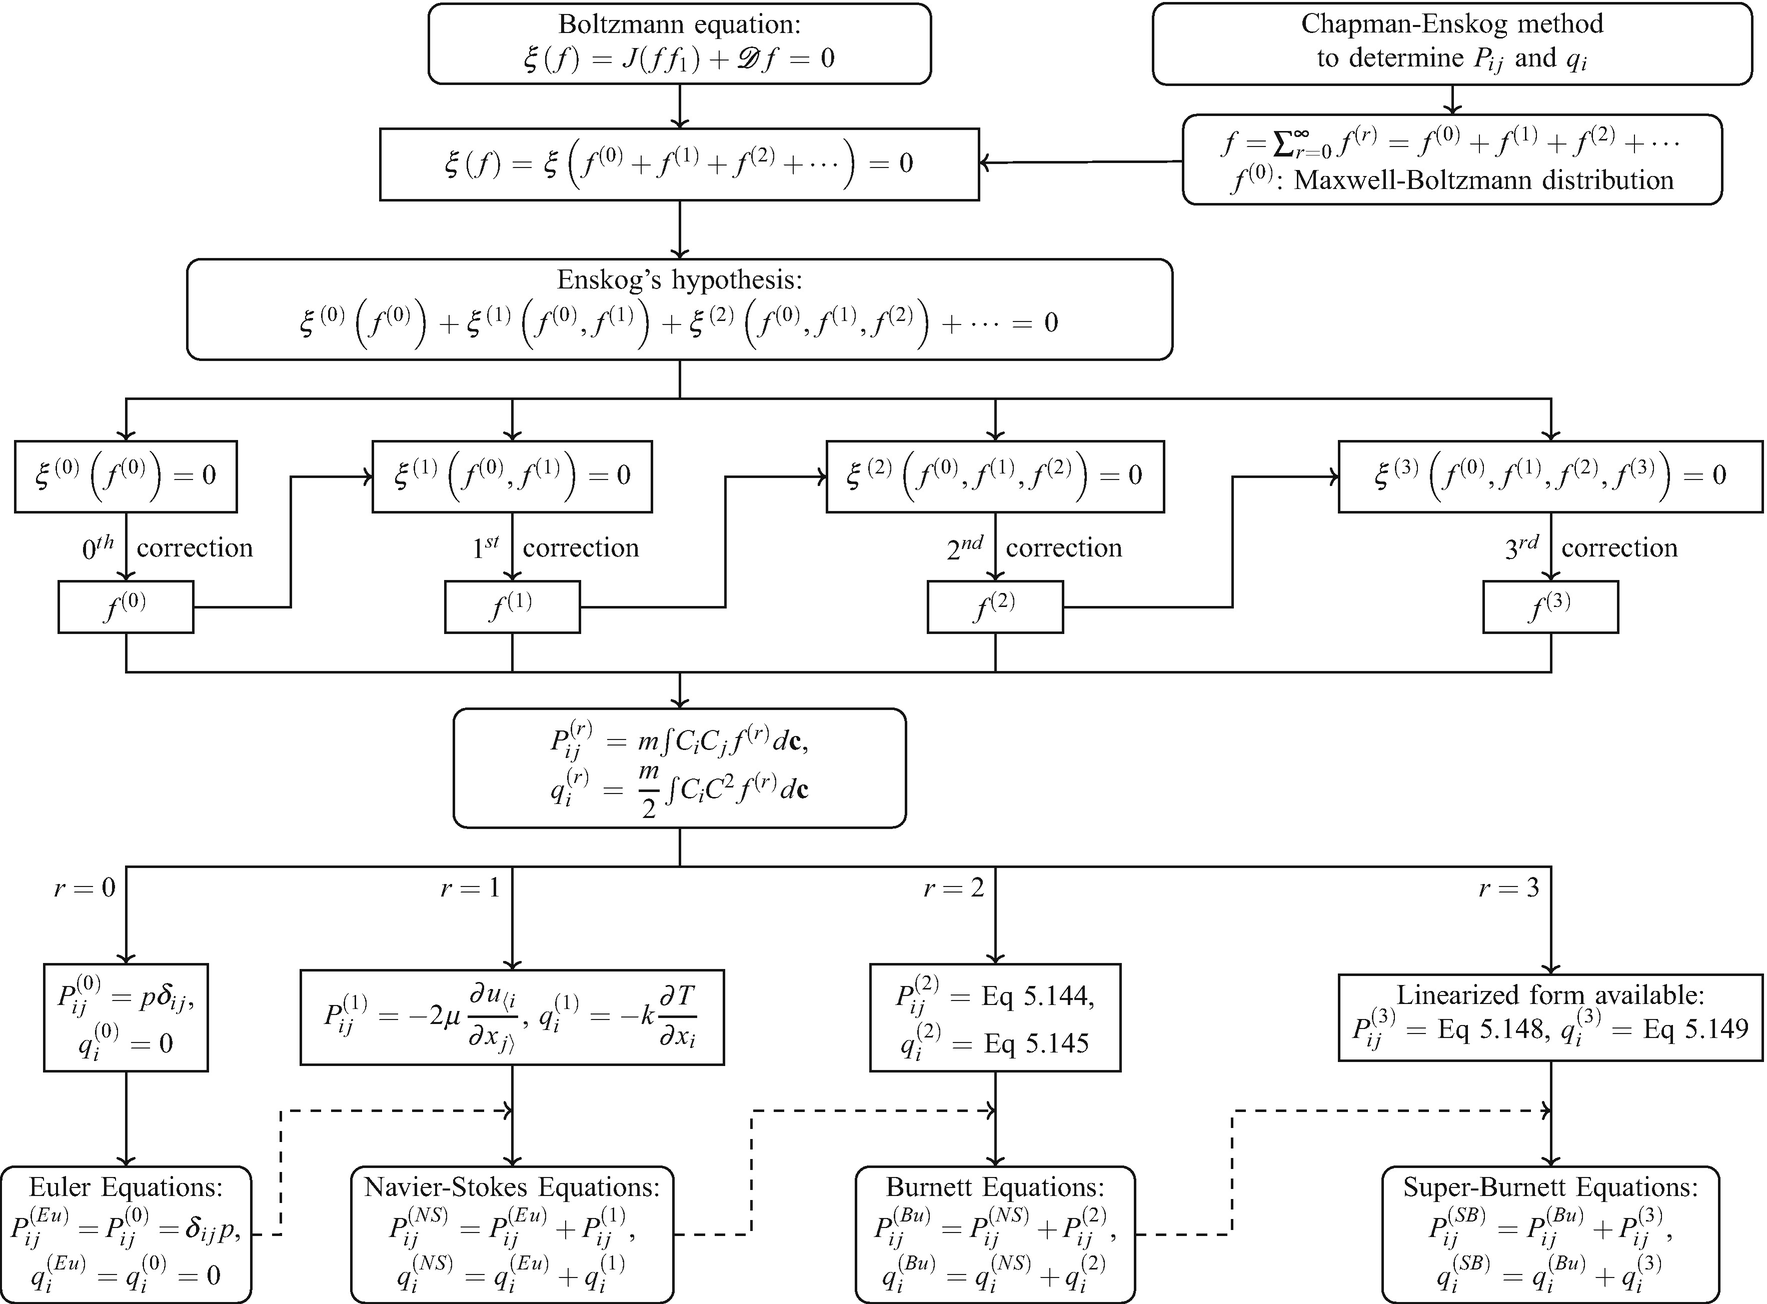
\includegraphics[width=0.9\textwidth]{../Images/2. Background/burnettflowchart.png}
    \caption{Flowchart of Burnett and Super Burnett equations derivation \cite{burnett}.}
    \label{fig:flowchart}
\end{figure}

It has been noted by the author that these equations, despite providing a correct analytical description of rarefied flows, are seldom to never used in literature for carrying out actual flow simulations. This is probably due to the existence of analytically simpler methods (which will be discussed in the following section), the difficulty of correctly computing accurate boundary conditions for Burnett equations and their linear instability to short wave disturbances \cite{comprarefied}.

\subsection{Rarefied flow simulation techniques}
Rarefied flow simulations are mainly divided into two categories: regular CFD codes with correction factors for velcoity slip and temperature jump, and Direct Simulation Monte Carlo solvers.



